
\chapter{Review}

\noindent This section covers the following ideas.


\begin{enumerate}

\item Graph basic functions by hand. Compute derivatives and integrals, in particular using the product rule, quotient rule, chain rule, integration by $u$-substitution, and integration by parts (the tabular method is useful for simplifying notation). Explain how to find a Laplace transform. 
\item Explain how to verify a function is a solution to an ODE, and illustrate how to solve separable ODEs.
\item Explain how to use the language of functions in high dimensions and how to compute derivatives using a matrix. Illustrate the chain rule in high dimensions with matrix multiplication.
\item Graph the gradient of a function together with several level curves to illustrate that the gradient is normal to level curves.
\item Explain how to test if a differential form is exact (a vector field is conservative) and how to find a potential. 

\end{enumerate}


\section{Basics}
You should understand how to graph by hand basic functions. If you have not spent much time graphing functions by hand, then please spend some time graphing the following functions:
$$x^2, x^3, x^4, \frac{1}{x}, \sin x, \cos x, \tan x, \arctan x, \ln x, e^x, e^{-x}$$
You should also practice shifting and rescaling function. For example the graph $\ds \frac{(x-h)^2}{a^2}+\frac{(y-k)^2}{b^2}=1$ is an ellipse shifted from the origin $h$ units right and $k$ units up. The graph of $y=2\sin x$ is formed by doubling the amplitude. The graph of $y=\sin(2x)$ if formed by halving the period. I suggest that you spend time graphing $y=A\sin(B(x-C))+D$ for various values of $A,B,C,D$ (for homework), and describe how each constant changes the shape of the function (the period is $\frac{2\pi}{B}$, amplitude is $A$, and the origin is moved from $(0,0)$ to $(C,D)$). 

\subsection{Derivatives}
You should know all the derivatives of the basic functions listed in the previous section.  In addition, you should know derivatives of the remaining trigonometric functions and trigonometric inverse functions (such as {$\arccos(x)$}), as well as rules regarding exponents {$a^x$} and logarithms {$\log_a x$} of any base.  The following rules are crucial as well.
\begin{enumerate}
	\item Power rule {$(x^n)^\prime = nx^{n-1}$}
	\item Sum and difference rule {$(f\pm g)^\prime = f^\prime\pm g^\prime$}
	\item Product and quotient rule {$(fg)^\prime = f g^\prime + f^\prime g$}
	\item Chain rule (arguably the most important) {$(f\circ g)^\prime = f^\prime(g(x))\cdot g^\prime(x)$}
\end{enumerate}
Be able to use the chain rule to do implicit differentiation. 

\begin{example} To find the derivative of {$\arcsin(x)$}, first rewrite the expression as {$x=\sin y$}.  Then differentiate both sides implicitly with respect to {$x$}, giving {$1=\cos(y) y^\prime$} (where the chain rule is used to get {$y^\prime$}).  Solving for {$y^\prime$} gives {$y^\prime = \frac{1}{\cos(y)}$}.  The expression {$x=\sin y$} means that {$y$} is the central angle of a triangle with {$x$} as the opposite edge and 1 as the hypotenuse.  This makes the adjacent edge {$\sqrt{1-x^2}$}.  Hence {$y^\prime = \frac{1}{\cos y} = \frac{1}{\sqrt{1-x^2}}$}.
\end{example}


\subsection{Integrals}
You should be able to integrate all the functions listed in the derivative section. In addition you should know the following integration techniques
\begin{itemize}
	\item {$u$}- substitution - The key is to pick the right {$u$}, solve for {$dx$}, and then compute the simpler integral.
	\begin{example} 
	To solve {$\int e^{3x}dx$}, first notice that we know how to integrate {$e^u$}, so let {$u=3x$}.  Then {$du = 3dx$}, or {$dx = \frac{du}{3}$}.  Substitution yields  {$\int e^{3x}dx=\int e^{u}\frac{du}{3} = \frac{1}{3}e^u+C=\frac{1}{3}e^{3x}+C$}. 
	\end{example}
	
\item Integration by parts - Recall the formula {$\int udv = uv-\int vdu$}. It is essentially the product rule (you can see that by differentiating both sides giving {$u dv = d(uv) - v du$}).  
\begin{example} 
To compute {$\int x\sin(2x)dx$}, we first pick for {$u$} a function which simplifies upon differentiation, and for {$dv$} the rest of the integrand.  The choice {$u=x$}, {$dv = \sin 2x dx$} will do.  This gives {$du = 1 dx$} and {$v = -\frac{\cos 2x}{2}$}.  Integration by parts gives {$\int x\sin(2x)dx = -x\frac{\cos 2x}{2} - \int -\frac{\cos 2x}{2} dx = -x\frac{\cos 2x}{2} + \frac{\sin 2x}{4}$}.
\end{example}

Integration by parts is needed to find the following integrals: $\int xe^xdx$, $\int x^2\sin x dx$, $\int e^x\sin x$, and $\int \ln x$. The Laplace Transform section will give you lots of practice with this.
\end{itemize}

There are other methods of integration, but we will only need to focus on integration by substitution and integration by parts. The following two sections illustrate the tabular method which is an organizational tool to help with integration by parts, and the Laplace transform which is one of the key tools used by engineers to solve ODEs. 

\subsubsection{The tabular method}
The tabular method is an organizational tool which simplifies integration by parts. This method gives you a convenient way to sort the information from multiple integration by parts into a simple table, so that you can find the integral without much work.

%An excellent article illustrating many uses of the tabular method.
%Tabular Integration by Parts
%David Horowitz, Golden West College, Huntington Beach, CA 92647
%The College Mathematics Journal, September 1990, Volume 21,
%Number 4, pp. 307�311.


\begin{example}
I'll illustrate this method with the same example as above, where $f(x)=x\sin(2x)$. 
Create a table with two sides. 
On the left side place a factor from your integral which will get simpler with differentiation. In this case we place $x$ on the left because after 2 derivatives it will become zero. On the right side place the rest of the integrand, which is $\sin(2x)$ in our example. 
\marginpar{{
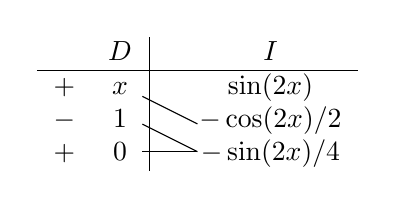
\begin{tikzpicture}
\begin{scope}[yshift=-3pt]
\draw (-.7,.2) -- (0,-.15);
\draw [yshift=-10pt] (-.7,.2) -- (0,-.15);
\draw [yshift=-10pt] (-.7,-.15) -- (0,-.15);
\end{scope}\path (0,0) node {
\begin{tabular}{cc|cc}
&$D$&&$I$\\\hline
$+$&$x$&&$\sin(2x)$\\
$-$&$1$&&$-\cos(2x)/2$\\
$+$&$0$&&$-\sin(2x)/4$\\
\end{tabular}};
\end{tikzpicture}}
}
Differentiate the left hand side one or more times. Stop differentiation when further differentiation will no longer simplify the problem. In this case we differentiated twice because we obtained 0. Now integrate the right side the same number of times. Multiply every other term on the left side by $-1$, starting with the second (this comes because of the minus in integration by parts, and you can see it in our table as the $+,-,+$ on the left of the table). Now multiply each term on the left by the term one row lower on the right (multiply diagonally down to the right), and sum the products. In our example we obtain $+(x)(-\cos(2x)/2)-(1)(-\sin(2x))$. The solution is found by add to the last step the integral of the product of the bottom row (if is zero, then this part can be skipped). In our case, the product of the bottom row is zero, so our solution is simply $\int x\sin(2x) =   +(x)(-\cos(2x)/2)-(1)(-\sin(2x))$.
\end{example}


\begin{example}
As another example let's compute $\int \ln x dx$. Since we don't know how to integrate $\ln x$, but we can differentiate it, we'll place $\ln x$ on the left side. Since there is nothing left in the integrand and $\ln x = \ln x \cdot 1$, we place a 1 on the right side.  The derivative of $\ln x$ is $1/x$.  The integral of $1$ is $x$.  Alternate the sign by placing a minus next to $1/x$.  
\marginpar{%\begin{center}
%\begin{wraptable}[5]{r}{0pt}
\begin{tabular}{cc|c}
&$D$&$I$\\\hline
$+$&$\ln x$&$1$\\
$-$&$1/x$&$x$\\
\end{tabular}
%\end{wraptable}
%\end{center}
}
Now multiply $\ln x$ by $x$ to obtain $x\ln x$.  The product of the bottom row is $-\frac{1}{x}x=-1$ so we add $\int -1 dx = -x$ to obtain $\int \ln x dx= x\ln x -x$.  
\end{example}


\subsubsection{Laplace Transforms}
The Laplace transform of a function $f(t)$ defined for $t\geq 0$ is $F(s)=L(f)=\int_0^\infty e^{-st}f(t)dt$, provided this improper integral exists (in which case we say the integral converges). Remember that to compute an improper integral you have to compute limits as the variable approaches infinity. The function $f(t)$ is called the inverse Laplace transform of $F(s)$, and we write $f(t)=L^{-1}(F)$. We will use the Laplace transform throughout the semester to help us solve many problems related to mechanical systems, electrical networks, and more. For now, we just need to know how to compute it (as it gives a good way to practice integration by parts)

If you have forgotten how to compute limits at infinity, then here is a brief review.  We can compute $\ds\lim_{t\to \infty} \frac{1}{t}=0$ since $\frac{1}{t}$ gets really small as $t$ gets large.  The function $e^{t}$ approaches $\infty$ as $t\to \infty$, but it approaches $0$ as $t\to -\infty$. This can be seen by looking at the graph of of $e^t$ which continues to increase forever as $t$ increases, but has a horizontal asymptote of $y=0$ as $t\to -\infty$. We will need to be able to compute limits such as $\ds\lim_{t\to\infty} te^{-st}=\lim_{t\to\infty} t\frac{t}{e^{st}}$. If you try taking the limits of both the top and bottom separately, you obtain $\frac{\infty}{\infty}$ (provided $s>0$). This is called an indeterminant form, and L'Hopital's rule says that you can examine such limits by taking the derivative of the top and the bottom separately and then taking a limit.  This gives $\ds\lim_{t\to\infty} \frac{t}{e^{-st}} = \lim_{t\to\infty} \frac{1}{(-s)e^{-st}} = \frac{1}{\infty} = 0$.


\begin{example}
If $f(t)=1$, then $F(s)=\int_0^\infty e^{-st}1dt= \frac{e^{-st}}{-s}\big|_0^\infty = \frac{1}{s}$, where the integral converges provided $s>0$. 
\end{example}
\begin{example}
If $f(t)=e^{at}$, then $F(s)=\int_0^\infty e^{-st}e^{at}dt=\int_0^\infty e^{-(s-a)t}dt= \frac{e^{-(s-a)t}}{-(s-a)}\big|_0^\infty = \frac{1}{s-a}$, where the integral converges provided $s>a$. 
\end{example}
\begin{example}
The Laplace transform of $t$ is $L(t)=F(s)=\int_0^\infty e^{-st}t dt$.  
Tabular integration by parts gives 
\marginpar{%\begin{center}
%\begin{wraptable}[5]{r}{0pt}
\begin{tabular}{cc|c}
&$D$&$I$\\\hline
$+$&$t$&$e^{-st}$\\
$-$&$1$&$e^{-st}/(-s)$\\
$+$&$0$&$e^{-st}/s^2$\\
\end{tabular}
%\end{wraptable}
%\end{center}
}
\begin{align*}
\ds L(t) 
&= \left[(t)(\frac{1}{-s}e^{-st}) - e^{-st}/s^2\right]\bigg|_0^\infty \\
&= \lim_{t\to \infty}\left(\frac{t}{-se^{-st}}-\frac{1}{s^2e^{-st}} \right) - (0-\frac{1}{s^2}) \\
&= (0-0)-(0-\frac{1}{s^2})=\frac{1}{s^2},
\end{align*}
where the integral converges if $s>0$. Similar computations show that $L(t^n) = \frac{n!}{s^{n+1}}, s>0$ for any integer $n$, where $n! = 1\cdot 2\cdot 3 \cdots n$ is the factorial function which is the product of all positive integers up to and including $n$. For example, $L(t^4) = \frac{4!}{s^5} = \frac{24}{s^5}$.
\end{example}

Since integration can be done term by term, we have $L(af+bg)=aL(f)+bL(g)$ for functions $f,g$ and constants $a,b$.  We can use this to find many other Laplace transforms without having to do any more integration. 
\begin{example}
Let's compute $L(4+6t-5e^{7t})$.  We distribute across each addition or subtraction sign to obtain $4L(1)+6L(t)-5L(e^{7t})$, and then using the results from the examples above we obtain $\frac{4}{s}+\frac{6}{s^2}-5\frac{1}{s-7}$. 
\end{example}
\begin{example}
Using the definition of $\ds\cosh t = \frac{e^t+e^{-t}}{2}$ and $\ds\sinh t = \frac{e^t-e^{-t}}{2}$, we can compute $$L(\cosh 3 t) = \frac{1}{2}L(e^{3t}+L(e^{-3t})) = \frac{1}{2}\left(\frac{1}{s-3}+\frac{1}{s+3}\right) = \frac{s}{s^2-3^2}.$$ Similarly $\ds L(\sinh 3 t) = \frac{3}{s^2-3^2}$. 
\end{example} 

%\begin{wraptable}[5]{r}{0pt}
%\begin{tabular}{|c|c|c|}
%\hline
%&$D$&$I$\\\hline
%$+$&$\cos \omega t$&$e^{-st}$\\
%$-$&$-\omega \sin \omega t$&$e^{-st}/(-s)$\\
%$+$&$-\omega^2 \cos \omega t$&$e^{-st}/s^2$\\\hline
%\end{tabular}
%\end{wraptable}
%
%Integration by parts twice yields $L(\cos \omega t) = \frac{s}{s^2+\omega^2}$ and $L(\sin \omega t) = \frac{\omega}{s^2+\omega^2}$. To see this, write $L(\cos \omega t) = \int_0^\infty e^{-st}\cos \omega t dt$.  The tabular method gives $\int_0^\infty e^{-st}\cos \omega t dt = \left(\cos \omega t e^{-st}/(-s) +\omega \sin \omega te^{-st}/s^2\right)\big|_0^\infty - \int_0^\infty \omega^2 \cos \omega te^{-st}/s^2dt = 1/s - \omega^2/s^2 \int_0^\infty e^{-st}\cos \omega t dt$, which means $L(\cos \omega t) = 1/s-\omega^2/s^2L(\cos \omega t)$. This means $(1+\omega^2/s^2)L(\cos \omega t) = \frac{1}{s}$, or $(s^2+\omega^2) L(\cos \omega t)=s$ or $L(\cos \omega t)=\frac{s}{s^2+\omega^2}$. You may discover that the ``trick'' of doing integration by parts twice can be very useful on integrals which involve sine, cosine, and exponential terms. 
%
%If a function is defined piecewise, then you have to break up your integral into multiple parts. For example, the Laplace transform of the function $f(t)=\begin{cases}2t&0\leq t\leq 4\\ 8 & 4<t<\infty \end{cases}$ is $L(f) = \int_0^\infty e^{-st}f(t)dt = \int_0^4 e^{-st} 2t dt +\int_4^\infty e^{-st}8 dt$.  The first integral (using integration by parts) is 
%$\int_0^4 e^{-st} 2t dt = \left[2t(\frac{1}{-s}e^{-st}) - 2e^{-st}/s^2\right]\bigg|_0^4 = (-\frac{8}{s}e^{-4s}-\frac{2}{s^2}e^{-4s})-(0-\frac{2}{s^2}) = \frac{2}{s^2} - (\frac{8}{s}+\frac{2}{s^2})e^{-4s}$.  The second integral is $\int_4^\infty e^{-st}8 dt= \frac{8}{-s}e^{-st}\bigg|_4^\infty = 0-\frac{8}{-s}e^{-4s} = \frac{8}{s}e^{-4s}$.  Adding these to together gives the Laplace transform of $f(t)$ as $F(s) = \frac{2}{s^2} - (\frac{8}{s}+\frac{2}{s^2})e^{-4s} + \frac{8}{s}e^{-4s}$.
%







\section{Ordinary Differential Equations}

A differential equation is an equation which involves derivatives (of any order) of some function.  For example, the equation $y^{\prime\prime}+xy^\prime+\sin(xy)=xy^2$ is a differential equation. An \textbf{ordinary differential equation (ODE)} is a differential equation involving an unknown function $y$ which depends on only one independent variable. The order of an ODE is the order of the highest derivative in the ODE. A solution to an ODE on an interval $(a,b)$ is a function $y(x)$ which satisfies the ODE on $(a,b)$. 
\begin{example}
The first order ODE $y^\prime = 2x$ has unknown function $y$ with independent variable $x$. A solution on $(-\infty,\infty)$ is the function $y=x^2+C$ for any constant $C$. The solution is found by simply integrating both sides. 
\end{example}
To verify that a function is a solution of an ODE, you just have to differentiate the function and then check to see if it satisfies the ODE.
\begin{example}
Let's verify that the function $y=\cos(2x)-3\sin(2x)$ satisfies (is a solution to) the 2nd order ODE $y^{\prime\prime}+4y=0$. We compute $y^\prime=-2\sin(2x)-6\cos(2x)$ and $y^{\prime\prime} = -4\cos(2x)+12\sin(2x)$.  We then put these into the ODE $y''+4y=0$ to obtain $-4\cos(2x)+12\sin(2x) + 4(\cos(2x)-3\sin(2x))=0$. Simplifying gives $0=0$, so we have verified that we have a solution.
\end{example}

Typically a solution to an ODE involves an arbitrary constant $C$. There is often an entire family of curves which satisfy a differential equation, and the constant $C$ just tells us which curve to pick. A \textbf{general solution} of an ODE is an infinite class of solutions of the ODE.  A \textbf{particular solution} is one of the infinitely many solutions of an ODE. Often an ODE comes with an \textbf{initial condition} $y(x_0)=y_0$ for some values $x_0$ and $y_0$. We can use these initial conditions to find a particular solution of the ODE. An ODE, together with an initial condition, is called an \textbf{initial value problem (IVP)}.  
\begin{example}
The IVP $y^\prime = 2x, y(2)=1$ has general solution $y=x^2+C$. Since $y=1$ when $x=2$, we have $1=2^2+C$ which means $C=-3$. Hence the solution to our IVP is $y=x^2-3$.
\end{example}

The most basic differential equation to solve is one in which you can ``separate'' the variables.  The idea is to rearrange the equation in the differential form $f(y)dy=g(x)dx$, where you separate the $x$ and $y$ terms so that they appear on different sides of the equation.  Integrating each side gives the general solution.

\begin{example}
Separate the ODE $y^\prime = \frac{x^2}{2y}$ by writing $2y \frac{dy}{dx} = x^2$ or $2ydy = x^2dx$. Integrating both sides gives a general solution $y^2 +C_1 = x^3/3 +C_2$, or simply $y^2 = x^3/3+C$ (since the difference of two arbitrary constants is just a constant). Here we can solve for $y$ to obtain $y=\pm\sqrt{x^3/3+C}$. Because we solved for $y$, we call this an explicit solution to the ODE. The solution $y^2 = x^3/3+C$ is called an implicit solution (where y is given implicitly rather than explicitly as a function of $x$).
\end{example}

\begin{example}
Divide the differential equation $y^\prime = ky$ on both sides by $y$. Then multiply both sides by the differential $dx$ to obtain $\frac{1}{y}dy = kdx$. Integration on both sides yields $\ln|y| = kx+c$.  Exponentiating both sides gives $|y|=e^{kx+c}=e^{kx}e^c$. Now $e^c$ is a positive constant, so we rename that constant to be $C$ and obtain $|y|=ce^{kx}$.  Removing the absolute values on $y$ just multiplies $C$ by $\pm 1$. This shows that the general solution to $y^\prime = ky$ is $y(x)=Ce^{kx}$.
\end{example}








\section{General Functions}
A function is a set of instructions (a relation) involving two sets (called the domain and range).  A function gives a rule that assigns to each element of the domain exactly one element in the range. It is customary to write {$f:D\to R$} when we want to specify exactly what the domain and range are. Often the domain and range are subsets of {${\mathbb{R}}^n$} (Euclidean {$n$}-space). If {$n=2$} then {${\mathbb{R}}^2$} is the coordinate plane. The domain and range do not have to be the same dimension. In multivariable calculus, you studied function of the form $f:{\mathbb{R}}^n\to  {\mathbb{R}}^m$ where $n$ and $m$ were 1, 2, or 3. The following list is provided as a reminder and summary of much of what you did in multivariable calculus.
\begin{enumerate}
	\item Functions of the form {$f:{\mathbb{R}}\to {\mathbb{R}}$} as in {$f(x)=x^2$} are studied in first semester calculus.

	\item Functions of the form {$f:{\mathbb{R}}\to {\mathbb{R}}^2$} as in {$\vec r(t) = \left<3\cos(t),2\sin(t)\right>$} are called parametric curves. They are plotted in the plane by making a $t,x,y$ table.

	\item Functions of the form {$f:{\mathbb{R}}\to {\mathbb{R}}^3$} as in {$\vec r(t) = \left<\cos(t),\sin(t),t\right>$} are called space curves. They are plotted in 3D by making a $t,x,y,z$ table.

	\item Functions of the form {$f:{\mathbb{R}}^2\to {\mathbb{R}}$} as in {$f(x,y)=9-x^2-y^2$} often represent surfaces, temperature, or density. We will use them to study differential equations. We often graph these as surfaces in 3D or use level curves (contour plots, isotherms (constant temperature), isobars (constant pressure) ) to describe these surfaces in 2D.

	\item Functions of the form {$f:{\mathbb{R}}^3\to {\mathbb{R}}$} as in {$f(x,y,z)=x^2+y^2+z^2$} are used to describe temperature, density, or other measurable quantities at every point in space. We graph with 3D level surfaces.

	\item Functions of the form {$f:{\mathbb{R}}^2\to {\mathbb{R}}^2$} or {$f:{\mathbb{R}}^3\to {\mathbb{R}}^3$} either represent vector fields or transformations. Think of polar, cylindrical, or spherical coordinate. Also think of gravity or some other force field, such as {$\vec F(x,y)=\left<-y,x\right>$} (counterclockwise rotation) or {$\vec F(x,y,z)=\left<x,y,z\right>$} (radial outward force). Graphs of planar vector fields $\vec F(x,y) = \left<M,N\right>$ are made by drawing the vector $\left<M,N\right>$ with its base at $(x,y)$. 

	\item Functions of the form {$f:{\mathbb{R}}^2\to {\mathbb{R}}^3$} such as {$\vec r(u,v)=\left<u,v,9-u^2-v^2\right>$} are called parametric surfaces. They are crucial to the development of electromagnetism and describing surfaces in space. We will not use them much in this class.

	\item Functions of the form {$f:{\mathbb{R}}^3\to {\mathbb{R}}^2$} such as {$\vec F(t,x,y)=\left<f_1,f_2\right>$} were not studied in multivariable calculus. They will be useful as we study mechanical systems and electrical networks.

\end{enumerate}


\subsection{General Derivatives}

Recall that to compute partial derivatives, we hold all but one variable constant and then differentiate with respect to that variable. Partial derivatives can be organized into a matrix $Df$ where each column represents the partial derivative of $f$ with respect to each variable.  This matrix, called the derivative or total derivative, takes us into our study of linear algebra. 
Some examples of functions and their derivatives appear in Table \ref{derivativetable}. When the output dimension is one, the matrix has only one row and the derivative is often called the gradient of $f$, written $\nabla f$.  

\begin{table}[htb]
\begin{center}
\begin{tabular}{|l|l|}
\hline
Function&Derivative\\ \hline\hline
{$f(x)=x^2$}& {$Df(x) = \begin{bmatrix}2x\end{bmatrix} $}\\ \hline
{$\vec r(t) = \left<3\cos(t),2\sin(t)\right>$}&  {$D\vec r(t) = \begin{bmatrix}-3\sin t\\ 2\cos t\end{bmatrix} $}\\ \hline
{$\vec r(t) = \left<\cos(t),\sin(t),t\right>$}&  {$D\vec r(t) = \begin{bmatrix}-\sin t \\ \cos t \\ 1\end{bmatrix} $}\\ \hline
{$f(x,y)=9-x^2-y^2$}&  {$Df(x,y) =\nabla f(x,y) = \begin{bmatrix}-2x & -2y\end{bmatrix} $}\\ \hline
{$f(x,y,z)=x^2+y+xz^2$}&  {$Df(x,y,z) = \nabla f(x,y,z) = \begin{bmatrix}2x+z^2 & 1 &2xz\end{bmatrix} $}\\ \hline
{$\vec F(x,y)=\left<-y,x\right>$}&  {$D\vec F(x,y) = \begin{bmatrix}0&-1\\ 1&0\end{bmatrix} $}\\ \hline
{$\vec F(r,\theta,z)=\left<r\cos\theta,r\sin\theta,z\right>$}&  {$D\vec F(r,\theta,z) = 
\begin{bmatrix}
\cos \theta &-r\sin\theta&0\\ 
\sin\theta&r\cos\theta&0\\ 
0&0&1
\end{bmatrix} $}\\ \hline
{$\vec r (u,v)=\left<u,v,9-u^2-v^2\right>$}&  {$D\vec r(u,v) = \begin{bmatrix}1&0\\ 0&1\\ -2u&-2v\end{bmatrix} $}\\ \hline
\end{tabular}
\end{center}
\caption{\label{derivativetable} The table above shows the (matrix) derivative of various functions.  Each column of the matrix corresponds a partial derivative of the function. When the output of a function is a vector, partial derivatives are vectors which are placed in columns of the matrix. The order of the columns matches the order in which you list the variables.}
\end{table}

In multivariate calculus, we focused our time on learning to graph and analyze each of these types of functions. As a review, I suggest that you practice drawing each of these types of functions, and remembering how to take their derivatives. 

\subsection{The General Chain Rule}
The chain rule in multivariable calculus is easy to remember if you understand matrix multiplication.  To multiply matrices $A$ and $B$, the $ij$th entry of the matrix is found by dotting the $i$th row of $A$ by the $j$th column of $B$. 
\begin{example} The product of a row matrix and a column matrix is simply the dot product of two vectors.  Notice that the number of columns of the first matrix must match the number of rows of the second matrix. 
$$ 
\begin{bmatrix}1 & 2\end{bmatrix}\begin{bmatrix}5\\6\end{bmatrix} =
\left<1 , 2\right>\cdot \left<5 , 6\right> = 1\cdot 5+ 2\cdot 6 = 17 
$$
\end{example}
\begin{example} For larger matrices, the new matrix is found by dotting each row with each column. The number of the row and the number of the column is the location of the dot product in the new matrix.
$$ 
\begin{bmatrix}1 &2\\3&4\end{bmatrix}\begin{bmatrix}5&0\\6&1\end{bmatrix} =
\begin{bmatrix}
\begin{bmatrix}1 &2\end{bmatrix}\begin{bmatrix}5\\6\end{bmatrix}
&\begin{bmatrix}1 &2\end{bmatrix}\begin{bmatrix}0\\1\end{bmatrix}
\\\begin{bmatrix}3&4\end{bmatrix}\begin{bmatrix}5 \\ 6\end{bmatrix}
&\begin{bmatrix}3&4\end{bmatrix}\begin{bmatrix}0 \\ 1\end{bmatrix}
\end{bmatrix}
=
\begin{bmatrix}5+12&0+2\\15+24&0+4\end{bmatrix}
=
\begin{bmatrix}17&2\\39&4\end{bmatrix}.$$
\end{example}
The chain rule in first semester calculus is {$(f\circ g)^\prime(x) = f^\prime (g(x))g^\prime(x)$}. Often we remember ``the derivative of the outside function times the derivative of the inside function.''  In multivariable calculus, often the formula {$\frac{df}{dt} = f_xx_t +f_yy_t$} is given for a function {$f(x,y)$}, where {$x$} and {$y$} depend on {$t$} (so that {$r(t)=\left<x(t),y(t)\right>$} is a curve traced out in the plane as $t$ increases). Written in matrix form, the chain rule is {$$\frac{df}{dt} = \begin{bmatrix}f_x&f_y\end{bmatrix}\begin{bmatrix}x_t\\ y_t\end{bmatrix} = Df\cdot Dr,$$} which is the (matrix) product of the derivatives, just as it was in first semester calculus. 

\begin{example}
Let {$f(x,y,z)=x^2+3y+5z$} where $x=u+v$, $y=u-v$, and $z=uv$. The equations for $x,y,$ and $z$ describe a parametric surface $\vec r (u,v)=\left<x,y,z\right> = \left<u+v,u-v,uv\right>$. The function $f\circ \vec r (u,v)$ describes how $f$ changes as $u$ or $v$ changes.  Hence we can ask what is $f_u$ and $f_v$. To find them, we use the chain rule and multiply the derivatives of $f$ and $\vec r$ together. The derivatives of $f$ and $\vec r$ are  $Df(x,y,z) = \begin{bmatrix}2x & 3 &5\end{bmatrix} $ and $D\vec r(u,v) = \begin{bmatrix}1&1\\ 1&-1\\ v&u\end{bmatrix} $.  The product is 
\begin{align*}
D(f\circ r)(u,v) &= DfDr \\
&= \begin{bmatrix}2x & 3 &5\end{bmatrix} \begin{bmatrix}1&1\\ 1&-1\\ v&u\end{bmatrix} \\
&= \begin{bmatrix}(2x)(1)+(3)(1)+5(v) & (2x)(1)+(3)(-1)+5(u)\end{bmatrix}\\
&= \begin{bmatrix}2(u+v)+3+5v & 2(u+v)-3+5u\end{bmatrix} \\
&= \begin{bmatrix}f_u & f_v\end{bmatrix} \\
\end{align*}
This gives the partial derivatives as
$f_u = \dfrac{\partial f}{\partial u} = 2(u+v)+3+5v$ and 
$f_v = \dfrac{\partial f}{\partial v} = 2(u+v)-3+5u$. The chain rule is simply matrix multiplication of the derivatives of each function.
\end{example}

\note{I would like to make this a theorem, and improve it to be an if and only if conditions. It's not hard to prove,  but for now I will postpone it.}
The chain rule proves the following key fact which we need as we study differential equations:  level curves of a function are orthogonal to the gradient. If $\vec r(t)$ is a level curve of $f$ (meaning $f\circ \vec r(t)=c$ for some constant $c$) then $D(f\circ r)(t) = 0$ since the value never changes, and by the chain rule $D(f\circ r)(t) = Df Dr = \nabla f \cdot r^\prime (t)$.  Combining these two facts gives $\nabla f\cdot r^\prime(t) = 0$. Since the dot product of these two vectors is zero, the vectors must be orthogonal. Hence the gradient of $f$ will be normal to the level curve.




\section{Gradient Fields, Potentials, Exact Differential Forms}
When the output dimension of a function is one, {$f:{\mathbb{R}}^n\to {\mathbb{R}}^1$}, the derivative is called the gradient, and written in vector form as {$\nabla f = \left<f_x,f_y,f_z\right>$}. If a vector field $\vec F = \left<M,N\right>$ (or in 3D $\vec F = \left<M,N,P\right>$) is the gradient of some some function $f$ (so that {$\nabla f= F$}), then we say that the vector field {$\vec F$} is a gradient field (or conservative vector field), and the function {$f$} is called  a potential for {$\vec F$}.  
\begin{example}
The gradient of $f(x,y)=9-x^2-y^2$ is $\nabla f = \left<-2x,-2y\right>$.  This is a vector field $\vec F = \left<-2x,-2y\right>$. 
So a potential for $\vec F = \left<-2x,-2y\right>$ is $f=9-x^2-y^2$, but another is just $f=-x^2-y^2$. 
\end{example}
How do we undo the differentiation process to find a potential? The point to this section is to review how to recognize when a vector has a potential (is a conservative vector field), and also how to find a potential. 

There is a test you can use to determine if a potential exists (it is often called the test for a conservative vector field).  If {$\vec F$} is a gradient field, then $\vec F = \left<f_x,f_y,f_z\right>$ for some $f$.  Since mixed partials must be equal (meaning $f_{xy}=f_{yx}$, $f_{xz}=f_{zx}$, and $f_{yz}=f_{zy}$), we can check to see if a vector field has a potential by checking if all three of the equations $M_y=N_x, M_z=P_x$, and $N_z=P_y$ hold. If one of these partial derivative pairs does not agree, then the vector field cannot be a gradient field. If these sets of partial derivatives do agree, then under reasonable conditions \note{a simply connnected domain} the vector field has a potential. 

\begin{example}
Consider the vector field $\left<x+yz,y+xz+z^2,xy+2yz+z^2\right>$. We compute 
$$\begin{array}{lll}
\left<x+yz\right.&,y+xz+z^2&,\left.xy+2yz+z^2\right>\\
M_y = z & N_x=z &P_x=y\\
M_z = y & N_z=x+2z &P_y=x+2z
\end{array}$$
and hence we know this vector field has a potential because $M_y=N_x, M_z=P_x$, and $N_z=P_y$. We'll show how to find a potential in a moment.
\end{example} 
 
The vocabulary of vector fields parallels the vocabulary of differential forms. A differential form is an expression of the form $Mdx+Ndy+Pdz$ (very similar to $\left<M,N,P\right>$).  
The differential of a function {$f$} is the expression {$df = f_xdx+f_ydy+f_zdz$} (similar to the gradient).  
\marginpar{A differential form is exact precisely when the corresponding vector field is a gradient field.} 
If a differential form is the differential of a function {$f$}, then the differential form is said to be exact (similar to saying a vector field is a gradient field). 
 Again, the function {$f$} is called  a potential for the differential form.  Notice that {$Mdx+Ndy+Pdz$} is exact if and only if {$\vec F = \left<M,N,P\right>$} is a gradient field. We will be using the language of differential forms throughout the semester. 
\begin{example}
The differential form $xdx+zdy+ydz$ is exact because the differential of $x^2/2+yz$ is $d(x^2/2+yz) = xdx+zdy+ydz$.  
\end{example}
\begin{example}
The differential form $-ydx+xdy$ is not exact because $M_y=-1$ does not equal $N_x=1$.
\end{example}

\subsection{How do you find a potential?} 
Consider the function $f =  x^2/2+xyz+ y^2/2+yz^2+z^3/3+25$.  Its differential is $df=(x+yz)dx+(y+xz+z^2)dy+(xy+2yz+z^2)dz$. If we erase $f$ and just keep the differential form $(x+yz)dx+(y+xz+z^2)dy+(xy+2yz+z^2)dz$, can we recover $f$? The first component $x+yz$ should equal $f_x$, so integrate it with respect to $x$.  Similarly, integrate the second component $y+xz+z^2$ with respect to $y$ and the third component $xy+2yz+z^2$ wit respect to $z$. 
These three integrals are 
\begin{align*}
&\int(x+yz)dx &&\int(y+xz+z^2)dy &&\int(xy+2yz+z^2)dz\\
&= \frac{x^2}{2}+xyz 
&&= \frac{y^2}{2}+xyz+yz^2 
&&= xyz+yz^2+\frac{z^3}{3}.
\end{align*}  
Notice that each integral contains an $xyz$ term, and the last two integrals both have a $yz^2$ term. The reason $xyz$ appears in each integral is that it has all three variables in it, and so its partial derivative with respect to all three variables is not zero.  The $yz^2$ does not appear in the first integral because it has no $x$ in it, and hence its partial derivative with respect to $x$ is zero.  A potential for $f$ is now obtained by adding together the three integrals, but realizing that you do not need to replicate the repeated terms.  A potential is hence $f(x,y,z) = x^2/2+xyz+ y^2/2+yz^2+z^3/3$. We did not recover the 25 from the original function. A potential is not unique; if a potential $f$ exists then $f+C$ is a potential for any constant $C$. 




\begin{example} Consider the vector field $\vec F=\left<2xy+x,x^2-3z,-3y+z^2\right>$. Since $M_y=2x=N_x,M_z=0=P_x,$ and $N_z=-3=P_y$, the field $\vec F$ has a potential. Integrate all three functions simultaneously, ignoring the constants, to get $\int M dx = x^2y+x^2/2 , \int N dy = x^2y+-3yz ,$ and $\int P dz = -3yz +z^3/3$. Since $x^2y$ and $-3yz$ appear in multiple integrals, we include them once in the sum to obtain for a potential $f= x^2y+x^2/2-3yz+z^3/3$.
\end{example}

\begin{example}
Consider the vector field $$\vec F(x,y,z) = \left<xy+yz+1,\frac12 x^2+xz-3z,xy-3y\right>.$$ The test for a conservative vector fields shows $M_y=x+z=N_x, M_z=y=P_x, N_z=x-3=P_y$, which means $\vec F$ is conservative.  A potential is found by integrating 
\begin{align*}
&\int xy+yz+1 dx &&\int \frac12 x^2+xz-3z dy &&\int xy-3y dz \\
&= \frac12x^2y+xyz+x 
&&=\frac12x^2y+xyz-3yz
&&= xyz-3yz.
\end{align*} The term $xyz$ appears in all three, $\frac12x^2y$ appears in the first and second, and $-3yz$ appears in the last two. A potential is found by summing the terms (ignoring repeats) to obtain $f(x,y,z) = \frac12x^2y+xyz+x-3yz$.  
\end{example}

%As a final review, the reason for the word ``potential'' comes from a study of potential energy and the fundamental theorem of line integrals.  The fundamental theorem of line integrals says that the work done by a conservative vector field $\vec F$ along a curve $C$ which starts at point $A$ and ends at point $B$ is equal to the change in the potential $f$ between these two points, or in symbolic notation we write $\ds\int_A^B \vec F \cdot d\vec r=\int_A^B Mdx+Ndy+Pdz = f(B)-f(A)$. The work done by the vector field $\vec F = \left<x,z,y\right>$ along any path which starts at the origin and ends at $(a,b,c)$ is written $\ds\int_{(0,0,0)}^{(a,b,c)}x dx + zdy + ydz$, since $f=x^2/2+yz$ is a potential for $\vec F$.  The fundamental theorem of line integrals says that this work equals $f(a,b,c)-f(0,0,0) = a^2-bc$.
